\chapter{建模与分析：从数据到周转圆}
\label{chap:modelling-analysis}
\markboth{建模与分析：从数据到周转圆}{建模与分析：从数据到周转圆}

\begin{remark}[本章目标的周期性判定（引用）]\label{rem:modelling_ps_hook}
本章判定研究目标是否具有周期性、确定其周期类型、以及查找最小正周期时，一律引用「周期系统」章：
周期性判据见 \cref{thm:ps_periodicity_decision}，
周期类型判别见 \cref{def:ps_period_type}、\cref{prop:ps_type_discrimination}，
最小正周期查找见 \cref{def:ps_minimal_period_algorithm}、\cref{thm:ps_minimal_period_correctness}，
由数据构建周期级数与周转圆组见 \cref{thm:ps_series_reconstruction}、\cref{def:ps_epicycle_group}。
\end{remark}

\begin{remark}[本章定位：从数据到周转圆的方法论枢纽]\label{rem:modelling_analysis_positioning}
本章建立周期数学的\textbf{统一方法论框架}——从实际问题建模、数据采集、周期分析、信号处理到模型评判，最终归结为周转圆模型及其复变函数实现。本章是连接周期数学理论体系（「级数与卷积」「调和分析」「周期系统」）与各应用领域（天文、历法、地理、生物、心理、经济、政治、算法、智能体）的\textbf{桥梁章节}。

核心方法论流程为：
\[
\boxed{\text{建模}} \to \boxed{\text{数据}} \to \boxed{\text{分析}} \to \boxed{\text{处理}} \to \boxed{\text{评判}} \to \boxed{\text{周期}} \to \boxed{\text{周转圆}} \to \boxed{\text{Waveform}}
\]
每一步都使用周期数学的核心工具：建模使用对称性与约束关系；数据采集使用动态采样理论（\cref{def:dynamic_sampling}）；分析使用周期卷积（\cref{def:periodic_convolution}）与相似度/趋势谱系（\cref{def:similarity_essence,def:tendency}）；处理使用窗函数（\cref{def:window_function}）和导-积下降优化（\cref{def:kdi_definition}）；评判使用信息准则（AIC/BIC）；周期识别使用周转圆嵌套生成（\cref{def:epicycle_nesting_rule}）；Waveform 作为复变函数使用复指数激活函数（\cref{def:epicycle-activation}）。

\textbf{本章的独特贡献}：将上述方法论框架同时以\textbf{数学陈述}与\textbf{编程建模（UML/图表）}两种方式表达。数学陈述给出严格的定理与证明；编程建模给出可实现的类体系、数据流、交互时序与业务过程。二者共同构成本章方法论的完整表达。

\textbf{本章七主题导引}：平移——数据采集的时间序列推进（\cref{def:data_acquisition}）与 Waveform 的时间平移不变性（\cref{prop:waveform_properties}）；缩放——BIC 的复杂度惩罚（\cref{ch34_pipeline_closure}）与多尺度窗函数（\cref{def:processing_tools}）；旋转——周转圆模型的相位 $\phi_k$（\cref{def:epicycle_modelling}）与 Waveform 的复变相位表示；平衡——BIC 拟合-复杂度平衡（\cref{prop:bic_balance}）与玻尔均值参数唯一性（\cref{ch34_epicycle_properties}）；对称——周转圆嵌套的层级对称；闭合——方法论流程的反馈迭代闭合（\cref{ch34_pipeline_closure}）与 Functor 类的闭包性质（\cref{prop:functor_closure}）；周期——频谱峰值识别（\cref{def:period_identification}）与周转圆参数估计（\cref{def:epicycle_modelling}）。
\end{remark}

\begin{remark}[本章的建模双轨制]\label{rem:modelling_dual_track}
本章对“建模与分析”采用\textbf{双轨制}表达：
\begin{enumerate}[label=(\roman*)]
    \item \textbf{数学轨道}：以定义、命题、引理、定理、推论、性质、例子、注释的严格顺序陈述并证明。数学轨道是本章的主干，所有结论必须可验证。
    \item \textbf{工程轨道}：以 Venn 图、甘特图、流程图、UML 图（上下文图、用例图、类图、对象图、时序图）、系统架构图、用户故事地图、业务过程模型、数据流图、ER 图等可视化工具表达。工程轨道是数学轨道的\textbf{辅助说明}——它不引入新的数学内容，只把数学轨道中的对象、关系、流程转化为可实现的工程语言。
\end{enumerate}
两条轨道的接口约定为：凡在工程轨道中出现的概念（如“Waveform”、“Epicycle”、“PeriodicSeries”），均已在数学轨道或前序章节给出严格定义；工程轨道中的图表\textbf{不构成新的数学断言}。这一约定保证了本章在不牺牲工程可实现性的同时，保持数学的严格性。
\end{remark}

\begin{lemma}[方法论流程的反馈闭合]\label{ch34_pipeline_closure}
设模型类 $\mathcal{M} = \{\mathcal{M}_K\}_{K=1}^{K_{\max}}$ 有限，其中 $K$ 为周转圆级数。评判指标为 BIC：
\[
\operatorname{BIC}(K) = n\ln(\operatorname{RSS}/n) + K\ln n,
\]
其中 $n$ 为样本量，$\operatorname{RSS}$ 为残差平方和。则“评判 $\to$ 反馈 $\to$ 重建模”的迭代按 BIC 严格下降，在有限步内收敛于 $\mathcal{M}$ 上的 BIC 最优模型。
\end{lemma}

\begin{proof}
反馈规则为：仅当 $\operatorname{BIC}(K') < \operatorname{BIC}(K)$ 时才用 $\mathcal{M}_{K'}$ 替换 $\mathcal{M}_K$。故每次迭代 BIC 严格下降。由于 $\mathcal{M}$ 有限（$K \le K_{\max}$），可能的 BIC 取值有限，严格下降序列必在有限步终止于某个 $K^*$。此时不存在使 BIC 更小的可替换模型，故 $\mathcal{M}_{K^*}$ 是 $\mathcal{M}$ 上的 BIC 最优模型。
\end{proof}

\section{方法论总览：上下文图与流程总图}

\subsection{上下文图：方法论与外部系统的边界}

\begin{figure}[htbp]
    \centering
    \adjustbox{max width=\textwidth}{%
    \begin{tikzpicture}[>=stealth,
        sys/.style={draw, rounded corners, fill=blue!15,
                    minimum width=4.2cm, minimum height=1.4cm,
                    align=center, font=\small\bfseries},
        ext/.style={draw, fill=gray!10,
                    minimum width=2.6cm, minimum height=0.9cm,
                    align=center, font=\footnotesize},
        arrow/.style={->, thick, >=stealth}]

        \node[sys] (sys) at (0,0) {周期数学\\建模与分析系统};

        \node[ext] (raw)  at (-5.5, 2.0) {原始数据\\（时间序列）};
        \node[ext] (know) at (-5.5, 0.0) {领域知识\\（对称性/约束）};
        \node[ext] (user) at (-5.5,-2.0) {建模者/工程师};

        \node[ext] (spec) at ( 5.5, 2.0) {频谱与相位\\结构化模型};
        \node[ext] (wf)   at ( 5.5, 0.0) {Waveform\\（复变函数）};
        \node[ext] (pred) at ( 5.5,-2.0) {预测与诊断\\（拐点/泄漏）};

        \draw[arrow] (raw)  -- (sys);
        \draw[arrow] (know) -- (sys);
        \draw[arrow] (user) -- (sys);

        \draw[arrow] (sys) -- (spec);
        \draw[arrow] (sys) -- (wf);
        \draw[arrow] (sys) -- (pred);

    \end{tikzpicture}%
    }
    \caption{周期数学建模与分析系统的上下文图。输入为原始时间序列、领域知识与建模者交互；
             输出为频谱与相位结构化模型、Waveform 复变函数表示、预测与诊断结果。}
    \label{fig:context_diagram}
\end{figure}

\newpage

\subsection{主流程图}

\begin{figure}[htbp]
    \centering
    \begin{tikzpicture}[>=stealth,
        box/.style={draw, rounded corners, minimum width=2.0cm, minimum height=0.9cm, align=center, font=\small},
        arrow/.style={->, thick, >=stealth}]
        
        \node[box, fill=blue!15] (model) at (0,0) {建模};
        \node[box, fill=green!15] (data) at (3,0) {数据};
        \node[box, fill=red!15] (analysis) at (6,0) {分析};
        
        \node[box, fill=orange!15] (processing) at (6,-2.2) {处理};
        \node[box, fill=purple!15] (evaluation) at (3,-2.2) {评判};
        
        \node[box, fill=yellow!15] (period) at (0,-4.4) {周期};
        \node[box, fill=cyan!15] (epicycle) at (3,-4.4) {周转圆};
        \node[box, fill=magenta!15] (waveform) at (6,-4.4) {Waveform};
        \node[box, fill=teal!15] (applications) at (9,-4.4) {应用};
        
        \draw[arrow] (model) -- (data);
        \draw[arrow] (data) -- (analysis);
        \draw[arrow] (analysis) -- (processing);  
        \draw[arrow] (processing) -- (evaluation);  
        \draw[arrow] (evaluation.west) -| (period.north);
        \draw[arrow] (period) -- (epicycle);
        \draw[arrow] (epicycle) -- (waveform);
        \draw[arrow] (waveform) -- (applications);
        
        \draw[arrow, dashed, blue, thick] (applications.south) to[out=-90, in=-90, looseness=1.5]
            node[below, font=\footnotesize] {反馈迭代} (model.south);
        
        \node[font=\footnotesize, text=blue!60!black]   at (0,-0.8) {对称性+约束};
        \node[font=\footnotesize, text=green!60!black]  at (3,-0.8) {动态采样};
        \node[font=\footnotesize, text=red!60!black]    at (6,-0.8) {周期卷积};
        \node[font=\footnotesize, text=orange!60!black] at (6,-3.0) {窗函数+导-积下降};
        \node[font=\footnotesize, text=purple!60!black] at (3,-3.0) {BIC+贝叶斯};
        
    \end{tikzpicture}
    \caption{周期数学统一方法论主流程图（蛇形回环布局）。第一行从左到右为建模、数据、分析；
             第二行从右到左为处理、评判；第三行从左到右为输出结构：周期、周转圆、Waveform、应用。
             虚线箭头表示从应用回到建模的反馈迭代。}
    \label{fig:methodology_main_flow}
\end{figure}

\newpage

\section{概念集合的 Venn 图}

\begin{figure}[htbp]
    \centering
    \begin{tikzpicture}[>=stealth, font=\small]

        \begin{scope}
            \draw[fill=blue!20,   opacity=0.45] (-1.0, 0.0) circle (1.25);
            \draw[fill=red!20,    opacity=0.45] ( 1.0, 0.0) circle (1.25);
            \draw[fill=green!20,  opacity=0.45] ( 0.0, 1.2) circle (1.25);

            \node[font=\small\bfseries, blue!70!black]  at (-2.7, -1.0) {平移 $P$};
            \node[font=\small\bfseries, red!70!black]   at ( 2.7, -1.0) {缩放 $S$};
            \node[font=\small\bfseries, green!70!black] at ( 0.0,  2.8) {旋转 $R$};

            \node[font=\scriptsize] at (-1.1,  0.8) {$P{\cap}R$};
            \node[font=\scriptsize] at ( 1.1,  0.8) {$S{\cap}R$};
            \node[font=\scriptsize] at ( 0.0, -0.8) {$P{\cap}S$};
            \node[font=\scriptsize] at ( 0.0,  0.4) {$P{\cap}S{\cap}R$};

            \node[font=\small\bfseries] at (0, -2.2) {(a) 三种基本变换};
        \end{scope}

        \begin{scope}[xshift=7cm]
            \draw[fill=blue!20,   opacity=0.45] (-1.0, 0.0) circle (1.25);
            \draw[fill=red!20,    opacity=0.45] ( 1.0, 0.0) circle (1.25);
            \draw[fill=green!20,  opacity=0.45] ( 0.0, 1.2) circle (1.25);

            \node[font=\small\bfseries, blue!70!black]  at (-2.7, -1.0) {$0$};
            \node[font=\small\bfseries, red!70!black]   at ( 2.7, -1.0) {$1$};
            \node[font=\small\bfseries, green!70!black] at ( 0.0,  2.8) {$i$};

            \node[font=\scriptsize] at (-1.1,  0.8) {$0{\cap}i$};
            \node[font=\scriptsize] at ( 1.1,  0.8) {$1{\cap}i$};
            \node[font=\scriptsize] at ( 0.0, -0.8) {$0{\cap}1$};
            \node[font=\scriptsize] at ( 0.0,  0.4) {$0{\cap}1{\cap}i$};

            \node[font=\small\bfseries] at (0, -2.2) {(b) 三种对称中心};
        \end{scope}

        \begin{scope}[yshift=-5.2cm, xshift=3.5cm]
            \draw[fill=orange!20, opacity=0.45] (-1.8, 0) circle (0.8);
            \draw[fill=cyan!20,   opacity=0.45] (-0.6, 0) circle (0.8);
            \draw[fill=purple!20, opacity=0.45] ( 0.6, 0) circle (0.8);
            \draw[fill=teal!20,   opacity=0.45] ( 1.8, 0) circle (0.8);

            \node[font=\scriptsize\bfseries, orange!70!black] at (-1.8, 0) {建模};
            \node[font=\scriptsize\bfseries, cyan!70!black]   at (-0.6, 0) {数据};
            \node[font=\scriptsize\bfseries, purple!70!black] at ( 0.6, 0) {分析};
            \node[font=\scriptsize\bfseries, teal!70!black]   at ( 1.8, 0) {处理};

            \node[font=\small] at (-1.2, 0.0) {$\cap$};
            \node[font=\small] at ( 0.0, 0.0) {$\cap$};
            \node[font=\small] at ( 1.2, 0.0) {$\cap$};

            \node[font=\small\bfseries] at (0, -2.2) {(c) 方法论四阶段};
        \end{scope}

    \end{tikzpicture}
    \caption{概念集合的 Venn 图。子图 (a) 中 $P$ 为平移、$S$ 为缩放、$R$ 为旋转，
             展示三种基本变换的两两交集 $P{\cap}S$、$P{\cap}R$、$S{\cap}R$
             与三重交集 $P{\cap}S{\cap}R$；
             子图 (b) 为三种对称中心（$0$ 加法、$1$ 乘法、$i$ 旋转）的交叠；
             子图 (c) 为方法论四阶段（建模、数据、分析、处理）相邻阶段的覆盖关系。
             Venn 图展示概念之间的重合与互补，不构成新的数学断言。}
    \label{fig:venn_concepts}
\end{figure}

\newpage

\section{建模工作流的甘特图}

\begin{figure}[htbp]
    \centering
    \begin{tikzpicture}[>=stealth, xscale=1.0, yscale=0.75]
        \draw[->] (0,0) -- (11,0) node[right, font=\footnotesize] {相对工作量};
        \foreach \x in {1,2,...,10} {
            \draw[gray!40] (\x,0) -- (\x,6.6);
            \node[font=\tiny, below] at (\x,0) {\x};
        }
        
        \filldraw[fill=blue!60, draw=blue!80] (0,6) rectangle (1.2,6.7);
        \node[font=\footnotesize, right] at (1.2,6.35) {建模：识别变换群与不变量};
        
        \filldraw[fill=green!60, draw=green!80] (1.2,5) rectangle (2.5,5.7);
        \node[font=\footnotesize, right] at (2.5,5.35) {数据：动态采样与预处理};
        
        \filldraw[fill=red!60, draw=red!80] (2.5,4) rectangle (5.0,4.7);
        \node[font=\footnotesize, right] at (5.0,4.35) {分析：FFT/周期卷积/相似度};
        
        \filldraw[fill=orange!60, draw=orange!80] (5.0,3) rectangle (7.5,3.7);
        \node[font=\footnotesize, right] at (7.5,3.35) {处理：窗函数平滑与拐点检测};
        
        \filldraw[fill=purple!60, draw=purple!80] (7.5,2) rectangle (9.0,2.7);
        \node[font=\footnotesize, right] at (9.0,2.35) {评判：BIC/AIC 模型选择};
        
        \filldraw[fill=cyan!60, draw=cyan!80] (9.0,1) rectangle (10.0,1.7);
        \node[font=\footnotesize, right] at (10.0,1.35) {输出：Waveform};
        
        \draw[->, thick, gray] (1.2,6.35) -- (1.2,5.35);
        \draw[->, thick, gray] (2.5,5.35) -- (2.5,4.35);
        \draw[->, thick, gray] (5.0,4.35) -- (5.0,3.35);
        \draw[->, thick, gray] (7.5,3.35) -- (7.5,2.35);
        \draw[->, thick, gray] (9.0,2.35) -- (9.0,1.35);
        
        \draw[->, thick, dashed, blue] (10.0,1.0) to[bend right=20] (0.3,6.3);
        \node[font=\footnotesize, blue!70!black] at (5,-0.9) {反馈迭代（\cref{ch34_pipeline_closure}）};
    \end{tikzpicture}
    \caption{建模工作流的甘特图。横轴为\textbf{相对工作量}（无量纲单位），不表示实际日历时间；纵向为任务序列。反馈迭代由 \cref{ch34_pipeline_closure} 保证有限步收敛。}
    \label{fig:gantt_workflow}
\end{figure}

\newpage

\section{用例图}

\begin{figure}[htbp]
    \centering
    \begin{tikzpicture}[
        >=stealth,
        usecase/.style={draw, ellipse, fill=blue!10, minimum width=2.8cm,
                        minimum height=0.85cm, align=center, font=\footnotesize},
        stickman/.pic={
            \draw[thick] (0,0.25) circle (0.15);
            \draw[thick] (-0.2,-0.05) -- (0.2,-0.05);
            \draw[thick] (0,0.10) -- (0,-0.30);
            \draw[thick] (-0.20,-0.55) -- (0,-0.30) -- (0.20,-0.55);
        }
    ]

        \coordinate (analyst)  at (-5, 3);
        \pic at (analyst)  {stickman};
        \node[font=\footnotesize] at (-5, 2.3) {建模者};

        \coordinate (engineer) at (-5, 0);
        \pic at (engineer) {stickman};
        \node[font=\footnotesize] at (-5, -0.7) {工程师};

        \coordinate (data)     at (-5, -3);
        \pic at (data)     {stickman};
        \node[font=\footnotesize] at (-5, -3.7) {数据源};

        \draw[thick, rounded corners] (-3, -4.2) rectangle (4, 4.2);
        \node[font=\small\bfseries] at (0.5, 3.9) {建模与分析系统};

        \node[usecase] (uc1) at (0.5,  3.0) {识别变换群};
        \node[usecase] (uc2) at (0.5,  2.0) {拟合周转圆参数};
        \node[usecase] (uc3) at (0.5,  1.0) {构建 Waveform};
        \node[usecase] (uc4) at (0.5,  0.0) {拐点与转折率诊断};
        \node[usecase] (uc5) at (0.5, -1.0) {相位耦合网络分析};
        \node[usecase] (uc6) at (0.5, -2.0) {模型选择（BIC/AIC）};
        \node[usecase] (uc7) at (0.5, -3.0) {采样与重采样};

        \draw (analyst)  -- (uc1);
        \draw (analyst)  -- (uc2);
        \draw (analyst)  -- (uc4);
        \draw (engineer) -- (uc3);
        \draw (engineer) -- (uc5);
        \draw (engineer) -- (uc6);
        \draw (data)     -- (uc7);

        \draw[dashed, ->] (uc3) -- node[right, font=\tiny] {$\ll$include$\gg$} (uc2);
        \draw[dashed, ->] (uc2) -- node[right, font=\tiny] {$\ll$include$\gg$} (uc7);

    \end{tikzpicture}
    \caption{建模与分析系统的用例图。三类参与者：建模者、工程师、数据源。
             核心用例包括识别变换群、拟合周转圆参数、构建 Waveform、
             拐点诊断、相位耦合分析、模型选择、采样与重采样。}
    \label{fig:use_case}
\end{figure}

\newpage

\section{用户故事地图}

\begin{figure}[htbp]
    \centering
    \begin{tikzpicture}[>=stealth,
        story/.style={draw, rounded corners, minimum width=2.5cm, minimum height=0.7cm, align=center, font=\tiny},
        header/.style={draw, rounded corners, fill=blue!15, minimum width=2.5cm, minimum height=0.7cm, align=center, font=\scriptsize\bfseries}]
        
        \node[header] (h1) at (0,4) {建模};
        \node[header] (h2) at (3,4) {数据};
        \node[header] (h3) at (6,4) {分析};
        \node[header] (h4) at (9,4) {处理};
        \node[header] (h5) at (12,4) {评判};
        
        \node[story, fill=blue!5] (s11) at (0,3.0) {识别对称群};
        \node[story, fill=blue!5] (s12) at (3,3.0) {动态采样};
        \node[story, fill=blue!5] (s13) at (6,3.0) {FFT};
        \node[story, fill=blue!5] (s14) at (9,3.0) {窗函数};
        \node[story, fill=blue!5] (s15) at (12,3.0) {BIC};
        
        \node[story, fill=green!5] (s21) at (0,2.1) {识别不变量};
        \node[story, fill=green!5] (s22) at (3,2.1) {预处理};
        \node[story, fill=green!5] (s23) at (6,2.1) {周期卷积};
        \node[story, fill=green!5] (s24) at (9,2.1) {拐点检测};
        \node[story, fill=green!5] (s25) at (12,2.1) {AIC};
        
        \node[story, fill=orange!5] (s31) at (0,1.2) {建立周期函数};
        \node[story, fill=orange!5] (s32) at (3,1.2) {尺度相关采样};
        \node[story, fill=orange!5] (s33) at (6,1.2) {相似度/趋势};
        \node[story, fill=orange!5] (s34) at (9,1.2) {转折率};
        \node[story, fill=orange!5] (s35) at (12,1.2) {交叉验证};
        
        \node[story, fill=red!5] (s41) at (0,0.3) {周转圆模型};
        \node[story, fill=red!5] (s42) at (3,0.3) {置闰};
        \node[story, fill=red!5] (s43) at (6,0.3) {相位耦合网络};
        \node[story, fill=red!5] (s44) at (9,0.3) {导-积下降};
        \node[story, fill=red!5] (s45) at (12,0.3) {残差诊断};
        
        \node[story, fill=purple!5] (s51) at (0,-0.6) {Waveform};
        \node[story, fill=purple!5] (s52) at (3,-0.6) {多通道};
        \node[story, fill=purple!5] (s53) at (6,-0.6) {周期卷积分解};
        \node[story, fill=purple!5] (s54) at (9,-0.6) {自适应窗};
        \node[story, fill=purple!5] (s55) at (12,-0.6) {贝叶斯选择};
        
        \draw[->, gray, dashed] (0,3.3) -- (0,3.5);
        \draw[->, gray, dashed] (3,3.3) -- (3,3.5);
        \draw[->, gray, dashed] (6,3.3) -- (6,3.5);
        \draw[->, gray, dashed] (9,3.3) -- (9,3.5);
        \draw[->, gray, dashed] (12,3.3) -- (12,3.5);
    \end{tikzpicture}
    \caption{用户故事地图。横轴为方法论的五大阶段（建模、数据、分析、处理、评判），纵轴为从基础能力到集成能力的故事层级。层级越高，故事覆盖的整合度越高；同一层级的故事可在该阶段独立交付。}
    \label{fig:user_story_map}
\end{figure}

\newpage

\section{业务过程模型（BPMN 风格）}

\begin{figure}[htbp]
    \centering
    \begin{tikzpicture}[>=stealth,
        start/.style={draw, circle, fill=green!40, minimum size=0.6cm},
        end/.style={draw, circle, fill=red!40, minimum size=0.6cm, double},
        task/.style={draw, rounded corners, fill=blue!10, minimum width=2.2cm, minimum height=0.7cm, align=center, font=\tiny},
        gateway/.style={draw, diamond, fill=yellow!30, minimum size=0.7cm, align=center, font=\tiny},
        arrow/.style={->, thick, >=stealth}]
        
        \node[start] (s) at (0,0) {};
        \node[task] (t1) at (2,0) {接收数据};
        \node[task] (t2) at (4.5,0) {周期检测};
        \node[gateway] (g1) at (7,0) {};
        \node[task] (t3) at (9.5,1.2) {拟合周转圆};
        \node[task] (t4) at (9.5,-1.2) {调整窗长};
        \node[task] (t5) at (12,0) {Waveform 输出};
        \node[end] (e) at (14,0) {};
        
        \draw[arrow] (s) -- (t1);
        \draw[arrow] (t1) -- (t2);
        \draw[arrow] (t2) -- (g1);
        \draw[arrow] (g1) -- node[left, font=\tiny, pos=0.5] {显著} (t3);
        \draw[arrow] (g1) -- node[left, font=\tiny, pos=0.5] {不显著} (t4);
        \draw[arrow] (t4) -- (t2);
        \draw[arrow] (t3) -- (t5);
        \draw[arrow] (t5) -- (e);
        
        \node[font=\tiny, above=0.1cm of g1] {峰值显著？};
    \end{tikzpicture}
    \caption{建模与分析的业务过程模型（BPMN 风格）。起于接收数据，经周期检测，若峰值显著则拟合周转圆并输出 Waveform；若不显著，调整窗长后重新检测，直至显著或达到终止条件。}
    \label{fig:bpmn}
\end{figure}

\newpage

\section{数据流图（DFD）}

\begin{figure}[htbp]
    \centering
    \begin{tikzpicture}[>=stealth,
        proc/.style={draw, rounded corners, fill=blue!10, minimum width=2.4cm, minimum height=0.9cm, align=center, font=\footnotesize},
        store/.style={draw, fill=gray!10, minimum width=2.4cm, minimum height=0.7cm, align=center, font=\footnotesize},
        ext/.style={draw, minimum width=2.0cm, minimum height=0.7cm, align=center, font=\footnotesize},
        arrow/.style={->, thick, >=stealth}]
        
        \node[ext]  (src) at (-4.5,  2.0) {数据源};
        \node[proc] (p1)  at (-1.5,  2.0) {采样与预处理};
        \node[proc] (p2)  at ( 1.5,  2.0) {频谱分析};
        
        \node[store] (ds1) at (-1.5, 0.5) {采样序列};
        \node[store] (ds2) at ( 1.5, 0.5) {频谱与相位};
        
        \node[proc] (p3)  at ( 1.5, -1.5) {周期卷积};
        \node[proc] (p4)  at (-1.5, -1.5) {导-积下降};
        \node[ext]  (out) at (-4.5, -1.5) {应用系统};
        
        \node[store] (ds3) at ( 1.5, -3.0) {相似度/趋势矩阵};
        \node[store] (ds4) at (-1.5, -4.0) {Waveform 参数};
        
        \draw[arrow] (src) -- (p1);
        \draw[arrow] (p1)  -- (p2);
        
        \draw[arrow] (p1)  -- (ds1);
        \draw[arrow] (ds1) -- (p2);
        
        \draw[arrow] (p2)  -- (ds2);
        \draw[arrow] (ds2) -- (p3);
        
        \draw[arrow] (p3)  -- (p4);
        \draw[arrow] (p4)  -- (out);
        
        \draw[arrow] (p3)  -- (ds3);
        
        \draw[arrow] (ds3.west) -| (p4.south);
        
        \draw[arrow] (p4)  -- (ds4);
        
        \draw[arrow] (ds4.west) -| (out.south);
        
    \end{tikzpicture}
    \caption{数据流图（DFD）。数据从数据源经采样与预处理、频谱分析、周期卷积、导-积下降到应用系统，中间存储为采样序列、频谱与相位、相似度/趋势矩阵、Waveform 参数。}
    \label{fig:dfd}
\end{figure}

\newpage

\section{ER 图}

\begin{figure}[htbp]
    \centering
    \begin{tikzpicture}[>=stealth,
        ent/.style={draw, fill=blue!10, minimum width=2.8cm, minimum height=0.8cm, align=center, font=\footnotesize\bfseries},
        attr/.style={draw, ellipse, fill=gray!10, minimum width=1.6cm, minimum height=0.6cm, align=center, font=\tiny},
        rel/.style={draw, diamond, fill=yellow!30, minimum size=0.8cm, align=center, font=\tiny},
        link/.style={thick}]
        
        \node[ent] (epi) at (0,3) {Epicycle};
        \node[ent] (wf) at (4,3) {Waveform};
        \node[ent] (ps) at (8,3) {PeriodicSeries};
        \node[ent] (sm) at (0,0) {Sample};
        \node[ent] (sp) at (4,0) {Spectrum};
        \node[ent] (sa) at (8,0) {Sampler};
        
        \node[attr] (a1) at (-2,4.2) {振幅 $A$};
        \node[attr] (a2) at (-2,2.6) {频率 $\omega$};
        \node[attr] (a3) at (0,4.6) {相位 $\phi$};
        
        \node[attr] (b1) at (4,4.6) {级数 $K$};
        \node[attr] (b2) at (6,4.2) {复变函数};
        
        \node[attr] (c1) at (8,4.6) {多周期};
        \node[attr] (c2) at (10,2.6) {分量集};
        
        \node[attr] (d1) at (-2,1) {采样值};
        \node[attr] (d2) at (0,-1) {采样率};
        
        \node[attr] (e1) at (4,1) {频率集};
        \node[attr] (e2) at (4,-1) {振幅集};
        
        \node[attr] (f1) at (8,1) {变换方法};
        
        \node[rel] (r1) at (2,3) {包含};
        \node[rel] (r2) at (6,3) {截断};
        \node[rel] (r3) at (2,0) {采样};
        \node[rel] (r4) at (6,0) {变换};
        
        \draw[link] (epi) -- (r1);
        \draw[link] (r1) -- (wf);
        \draw[link] (wf) -- (r2);
        \draw[link] (r2) -- (ps);
        \draw[link] (sm) -- (r3);
        \draw[link] (r3) -- (sp);
        \draw[link] (sp) -- (r4);
        \draw[link] (r4) -- (sa);
        
        \draw[thin] (epi) -- (a1);
        \draw[thin] (epi) -- (a2);
        \draw[thin] (epi) -- (a3);
        \draw[thin] (wf) -- (b1);
        \draw[thin] (wf) -- (b2);
        \draw[thin] (ps) -- (c1);
        \draw[thin] (ps) -- (c2);
        \draw[thin] (sm) -- (d1);
        \draw[thin] (sm) -- (d2);
        \draw[thin] (sp) -- (e1);
        \draw[thin] (sp) -- (e2);
        \draw[thin] (sa) -- (f1);
    \end{tikzpicture}
    \caption{ER 图。六类实体：Epicycle（周转圆）、Waveform（复变函数）、PeriodicSeries（周期级数）、Sample（采样）、Spectrum（频谱）、Sampler（变换器）。关系为包含、截断、采样、变换。}
    \label{fig:er_diagram}
\end{figure}

\newpage

\section{系统架构图}

\begin{figure}[htbp]
    \centering
    \begin{tikzpicture}[>=stealth,
        layer/.style={draw, rounded corners, minimum width=12cm, minimum height=1.2cm, align=center, font=\small},
        comp/.style={draw, rounded corners, fill=white, minimum width=2.2cm, minimum height=0.7cm, align=center, font=\tiny},
        arrow/.style={->, thick, >=stealth}]
        
        \node[layer, fill=blue!10] (L1) at (0,4) {\textbf{应用层（Application）}\\ 天文、历法、地理、生物、心理、经济、政治、算法、智能体};
        \node[layer, fill=green!10] (L2) at (0,2.5) {\textbf{建模与分析层（Modelling \& Analysis）}\\ 周期卷积、相似度/趋势、导-积下降};
        \node[layer, fill=orange!10] (L3) at (0,1) {\textbf{数据结构层（Data Structure）}\\ Epicycle、Waveform、PeriodicSeries、Spectrum};
        \node[layer, fill=purple!10] (L4) at (0,-0.5) {\textbf{基础算符层（Primitive Operators）}\\ FFT、梅林、拉普拉斯、Chirp-Z、小波、周期变换};
        \node[layer, fill=red!10] (L5) at (0,-2) {\textbf{采样与观察层（Sampling \& Observer）}\\ 动态采样、置闰、奈奎斯特、尺度相关};
        
        \draw[arrow] (L1.south) -- (L2.north);
        \draw[arrow] (L2.south) -- (L3.north);
        \draw[arrow] (L3.south) -- (L4.north);
        \draw[arrow] (L4.south) -- (L5.north);
        
        \node[font=\tiny, right=0.2cm of L1] {(API)};
        \node[font=\tiny, right=0.2cm of L2] {(Algorithms)};
        \node[font=\tiny, right=0.2cm of L3] {(Classes)};
        \node[font=\tiny, right=0.2cm of L4] {(Transforms)};
        \node[font=\tiny, right=0.2cm of L5] {(Hardware)};
    \end{tikzpicture}
    \caption{系统架构图。五层架构：应用层、建模与分析层、数据结构层、基础算符层、采样与观察层。层间依赖由下而上单向。}
    \label{fig:architecture}
\end{figure}

\newpage

\section{核心类的程序表示}

本节将周期数学的核心概念映射为程序表示。核心抽象是 \textbf{Functor}——所有光滑（$C^\infty$）的、可反复求导与积分的数学对象。类体系分为三个模块：函数类层次结构、级数类层次结构、积分变换与采样类。

\subsection{Functor 类：光滑函数的抽象基类}

\begin{definition}[Functor 类]\label{def:functor_class}
\textbf{Functor} 是所有光滑函数（即 $C^\infty$ 函数）的抽象基类。其核心方法为求导、积分、极限与求值：
\begin{enumerate}[label=(\roman*)]
    \item \texttt{derivative(t)}：返回 Functor 在 $t$ 处的导数——仍是一个 Functor。
    \item \texttt{integral(t)}：返回 Functor 的不定积分（原函数）——仍是一个 Functor。
    \item \texttt{integral(a, b)}：返回 Functor 在区间 $[a,b]$ 上的定积分（面积）。
    \item \texttt{limit(t)}：返回 Functor 在 $t$ 处的极限值。
    \item \texttt{evaluate(t)}：返回 Functor 在 $t$ 处的函数值。
\end{enumerate}
Functor 的子类包括：线性函数、二次函数、三次函数、正弦函数、余弦函数、正切函数、Epicycle、Waveform、Convolution 以及 Series。
\end{definition}

\begin{property}[Functor 类的闭包性质]\label{prop:functor_closure}
Functor 类在以下运算下封闭：
\begin{enumerate}[label=(\roman*)]
    \item \textbf{微分}：Functor 的导数仍是 Functor。
    \item \textbf{积分}：Functor 的原函数仍是 Functor。
    \item \textbf{线性组合}：两个 Functor 的线性组合仍是 Functor。
    \item \textbf{复合}：两个 Functor 的复合仍是 Functor。
    \item \textbf{卷积}：两个 Functor 的卷积仍是 Functor。
\end{enumerate}
\end{property}

\begin{proof}
(i)(ii) 由微积分基本定理，$C^\infty$ 函数的导数和原函数仍是 $C^\infty$ 函数。
(iii) 线性组合的导数等于导数的线性组合，故仍是 Functor。
(iv) 由链式法则，复合函数的导数存在且可计算。
(v) 由卷积的微分性质 $(f * g)' = f' * g = f * g'$，卷积仍是 $C^\infty$ 函数。
\end{proof}

\subsection{函数类层次结构}

\begin{definition}[基本函数子类]\label{def:basic_function_subclasses}
Functor 的基本子类包括：
\begin{enumerate}[label=(\roman*)]
    \item \textbf{LinearFunction}：$f(t) = at + b$，导数为常数 $a$，原函数为 $\frac{a}{2}t^2 + bt + C$。
    \item \textbf{QuadraticFunction}：$f(t) = at^2 + bt + c$，导数为 $2at + b$。
    \item \textbf{CubicFunction}：$f(t) = at^3 + bt^2 + ct + d$。
    \item \textbf{SineFunction}：$f(t) = A\sin(\omega t + \phi)$，导数为 $A\omega\cos(\omega t + \phi)$。
    \item \textbf{CosineFunction}：$f(t) = A\cos(\omega t + \phi)$，导数为 $-A\omega\sin(\omega t + \phi)$。
    \item \textbf{TangentFunction}：$f(t) = A\tan(\omega t + \phi)$，导数为 $A\omega\sec^2(\omega t + \phi)$。
\end{enumerate}
\end{definition}

\begin{proposition}[基本函数的导数封闭性]\label{prop:basic_function_derivative_closure}
基本函数子类在微分运算下的封闭关系为：
\begin{enumerate}[label=(\roman*)]
    \item $\frac{d}{dt}\operatorname{Sine}(\omega t) = \omega \cdot \operatorname{Cosine}(\omega t)$。
    \item $\frac{d}{dt}\operatorname{Cosine}(\omega t) = -\omega \cdot \operatorname{Sine}(\omega t)$。
    \item $\frac{d}{dt}\operatorname{Tangent}(\omega t) = \omega \cdot \operatorname{Secant}^2(\omega t)$。
\end{enumerate}
正弦与余弦在微分下相互转换，构成 $2$-周期闭轨道。
\end{proposition}

\begin{proof}
由基本导数公式直接验证。正弦函数求导得余弦函数，余弦函数求导得负正弦函数，两次求导后回到自身（相差负号），构成 $C_2$ 对合结构（\cref{def:group_action}）。
\end{proof}

\begin{definition}[Epicycle 类]\label{def:epicycle_class}
\textbf{Epicycle} 类继承自 Functor，表示单个周转圆：
\[
\gamma(t) = A e^{i(\omega t + \phi)}.
\]
其字段为振幅 $A$、角频率 $\omega$、初始相位 $\phi$。Epicycle 是周期数学中最基本的几何单元，也是 Waveform 的组成元素（其数学对象即 \cref{def:epicycle}）。
\end{definition}

\begin{property}[Epicycle 类的方法语义]\label{prop:epicycle_class_methods}
\begin{enumerate}[label=(\roman*)]
    \item \texttt{derivative(t)}：返回 $\omega A e^{i(\omega t + \phi + \pi/2)}$——振幅乘以 $\omega$，相位增加 $\pi/2$。
    \item \texttt{integral(t)}：返回 $\frac{A}{\omega} e^{i(\omega t + \phi - \pi/2)}$——振幅除以 $\omega$，相位减少 $\pi/2$。
    \item \texttt{integral(a, b)}：返回 $\frac{A}{i\omega}(e^{i(\omega b + \phi)} - e^{i(\omega a + \phi)})$。
    \item \texttt{evaluate(t)}：返回 $A e^{i(\omega t + \phi)}$。
    \item \texttt{convolute(Epicycle, Delay)}：返回两个 Epicycle 在给定时延下的周期卷积（\cref{def:periodic_convolution}）。
    \item \texttt{similarity(Epicycle)}：返回两个 Epicycle 的相似度（\cref{def:similarity_essence}）。
    \item \texttt{tendency(Epicycle)}：返回两个 Epicycle 的趋势（\cref{def:tendency}）。
\end{enumerate}
\end{property}

\begin{proof}
导数：$\frac{d}{dt}Ae^{i(\omega t + \phi)} = i\omega A e^{i(\omega t + \phi)} = \omega A e^{i(\omega t + \phi + \pi/2)}$。
积分：$\int Ae^{i(\omega t + \phi)}dt = \frac{A}{i\omega}e^{i(\omega t + \phi)} = \frac{A}{\omega}e^{i(\omega t + \phi - \pi/2)}$。
定积分由微积分基本定理直接给出。卷积、相似度和趋势由 \cref{def:periodic_convolution,def:similarity_essence,def:tendency} 的定义逐分量计算。
\end{proof}

\begin{definition}[Waveform 类]\label{def:waveform_class}
\textbf{Waveform} 类继承自 Functor，表示由多个 Epicycle 组成的复变函数（其数学对象即 \cref{def:waveform_definition}）：
\[
\mathcal{W}(t) = \sum_{k=1}^{K} A_k e^{i(\omega_k t + \phi_k)}.
\]
其内部使用双端队列存储 Epicycle 对象。Waveform 既是 Functor（可求导、可积分），又是 Epicycle 的容器（可添加、删除周转圆）。
\end{definition}

\begin{property}[Waveform 类的方法语义]\label{prop:waveform_class_methods}
\begin{enumerate}[label=(\roman*)]
    \item 队列操作：\texttt{pushFront}、\texttt{removeFront}、\texttt{pushBack}、\texttt{removeBack}、\texttt{removeAt}——支持周转圆的动态添加和删除。
    \item \texttt{front()} / \texttt{back()}：返回第一个或最后一个 Epicycle。
    \item Functor 接口：\texttt{derivative(t)}、\texttt{integral(t)}、\texttt{integral(a,b)}、\texttt{limit(t)}、\texttt{evaluate(t)}——逐分量作用于每个 Epicycle。
    \item \texttt{convolute(Waveform, Delay)}：返回两个 Waveform 的周期卷积。
    \item \texttt{similarity(Waveform)}：返回两个 Waveform 的相似度矩阵。
    \item \texttt{tendency(Waveform)}：返回两个 Waveform 的趋势矩阵。
\end{enumerate}
\end{property}

\begin{proof}
Waveform 的 Functor 方法是 Epicycle 对应方法的逐分量推广。由于 Waveform 是 Epicycle 的有限和，线性运算（微分、积分）可以逐分量进行。卷积、相似度和趋势由 \cref{def:periodic_convolution,def:similarity_essence,def:tendency} 的定义逐分量计算。
\end{proof}

\begin{definition}[Convolution 类]\label{def:convolution_class}
\textbf{Convolution} 类继承自 Functor，表示两个 Functor 的卷积：
\[
(f * g)(t) = \int_{-\infty}^{\infty} f(\tau) g(t - \tau) d\tau.
\]
Convolution 本身是一个 Functor——可求导、可积分。其数学对象即 \cref{def:convolution}。
\end{definition}

\begin{property}[Convolution 类的微分性质]\label{prop:convolution_class_derivative}
\[
(f * g)' = f' * g = f * g'.
\]
卷积的导数等于任一因子的导数与另一因子的卷积。
\end{property}

\begin{proof}
由 \cref{prop:convolution_properties}(v) 直接得出。这是卷积作为 Functor 的关键性质——它保证了卷积在 Functor 类中的封闭性。
\end{proof}

\newpage

\begin{figure}[htbp]
    \centering
    \begin{tikzpicture}[>=stealth,
        classbox/.style={draw, rectangle, minimum width=2.8cm, align=left, font=\scriptsize, inner sep=4pt},
        inherit/.style={->, thick, >=open triangle 60, dashed}]
        
        \node[classbox, fill=orange!10, minimum height=1.2cm] (linear) at (-4.0,5.0) {\textbf{LinearFunction}\\ \texttt{+ a, b}};
        \node[classbox, fill=orange!10, minimum height=1.2cm] (quadratic) at (0,5.0) {\textbf{QuadraticFunction}\\ \texttt{+ a, b, c}};
        \node[classbox, fill=orange!10, minimum height=1.2cm] (cubic) at (4.0,5.0) {\textbf{CubicFunction}\\ \texttt{+ a, b, c, d}};
        
        \node[classbox, fill=orange!10, minimum height=1.2cm] (exponential) at (-6,1.5) {\textbf{ExponentialFunction}\\ \texttt{+ base}};
        \node[classbox, fill=orange!10, minimum height=1.2cm] (logarithmic) at (-6,0) {\textbf{LogarithmicFunction}\\ \texttt{+ base}};
        \node[classbox, fill=orange!10, minimum height=1.2cm] (power) at (-6,-1.5) {\textbf{PowerFunction}\\ \texttt{+ exponent}};
        
        \node[classbox, fill=gray!10, minimum height=2.8cm] (functor) at (0,0) {
            \textbf{Functor}\\[2pt]
            \texttt{+ derivative(t)}\\
            \texttt{+ integral(t)}\\
            \texttt{+ integral(a, b)}\\
            \texttt{+ limit(t)}\\
            \texttt{+ evaluate(t)}
        };
        
        \node[classbox, fill=orange!10, minimum height=1.2cm] (sine) at (6,1.5) {\textbf{SineFunction}\\ \texttt{+ A, omega, phi}};
        \node[classbox, fill=orange!10, minimum height=1.2cm] (cosine) at (6,0) {\textbf{CosineFunction}\\ \texttt{+ A, omega, phi}};
        \node[classbox, fill=orange!10, minimum height=1.2cm] (tangent) at (6,-1.5) {\textbf{TangentFunction}\\ \texttt{+ A, omega, phi}};
        
        \node[classbox, fill=blue!10, minimum height=1.8cm] (epicycle) at (-4.0,-4.5) {
            \textbf{Epicycle}\\[2pt]
            \texttt{+ amplitude}\\
            \texttt{+ omega}\\
            \texttt{+ phase}
        };
        
        \node[classbox, fill=green!10, minimum height=1.8cm] (waveform) at (0,-4.5) {
            \textbf{Waveform}\\[2pt]
            \texttt{+ epicicles}\\
            \texttt{+ push / remove}\\
            \texttt{+ convolute}\\
            \texttt{+ similarity}\\
            \texttt{+ tendency}
        };
        
        \node[classbox, fill=red!10, minimum height=1.8cm] (convolution) at (4.0,-4.5) {
            \textbf{Convolution}\\[2pt]
            \texttt{+ f : Functor}\\
            \texttt{+ g : Functor}
        };
        
        \draw[inherit] (linear.south) -- (functor.north);
        \draw[inherit] (quadratic.south) -- (functor.north);
        \draw[inherit] (cubic.south) -- (functor.north);
        \draw[inherit] (exponential.east) -- (functor.west);
        \draw[inherit] (logarithmic.east) -- (functor.west);
        \draw[inherit] (power.east) -- (functor.west);
        \draw[inherit] (sine.west) -- (functor.east);
        \draw[inherit] (cosine.west) -- (functor.east);
        \draw[inherit] (tangent.west) -- (functor.east);
        \draw[inherit] (epicycle.north) -- (functor.south);
        \draw[inherit] (waveform.north) -- (functor.south);
        \draw[inherit] (convolution.north) -- (functor.south);
        \draw[->, thick, >=stealth] (waveform.west) -- node[above, font=\tiny] {包含} (epicycle.east);
    \end{tikzpicture}
    \caption{函数类层次结构（UML 类图）。Functor 是所有可微函数的抽象基类。上方为代数函数（线性、二次、三次），左方为超越函数（指数、对数、幂），右方为三角函数（正弦、余弦、正切），下方为周期数学核心类（Epicycle、Waveform、Convolution）。Waveform 包含 Epicycle 的集合。}
    \label{fig:uml_functor_hierarchy}
\end{figure}

\newpage

\subsection{级数类层次结构}

\begin{definition}[Series 类]\label{def:series_class}
\textbf{Series} 类继承自 Functor，表示函数项级数：
\[
S(t) = \sum_{k=0}^{\infty} u_k(t).
\]
其字段为项序列 \texttt{terms: Deque<Functor>} 和展开中心 \texttt{center: Number}。Series 的子类包括泰勒级数、傅里叶级数、洛朗级数和周期级数。
\end{definition}

\begin{property}[Series 类的方法语义]\label{prop:series_class_methods}
\begin{enumerate}[label=(\roman*)]
    \item \texttt{evaluate(t)}：返回级数在 $t$ 处的部分和（取前 $n$ 项）。
    \item \texttt{truncate(n)}：返回截断到前 $n$ 项的级数。
    \item \texttt{derivative(t)}：逐项求导，返回新的 Series。
    \item \texttt{integral(t)}：逐项积分，返回新的 Series。
    \item \texttt{convergeRadius()}：返回级数的收敛半径（对泰勒/洛朗级数；对傅里叶/周期级数返回 $\infty$ 或按周期长度定义）。
\end{enumerate}
\end{property}

\begin{proof}
级数的逐项求导和逐项积分由一致收敛性保证（\cref{thm:uniform_termwise_integration,thm:uniform_termwise_differentiation}）。收敛半径由柯西-阿达马公式（\cref{thm:cauchy_hadamard}）计算。
\end{proof}

\begin{definition}[泰勒级数程序表示]\label{def:taylor_series_class}
该类所表示的数学对象即 \cref{def:taylor_series} 定义的泰勒级数；此处只给出其程序表示（类名与继承关系），不重新定义数学对象。\textbf{TaylorSeries} 继承自 Series，表示函数在 $t_0$ 处的泰勒展开：
\[
f(t) = \sum_{k=0}^{\infty} \frac{f^{(k)}(t_0)}{k!}(t - t_0)^k.
\]
\end{definition}

\begin{definition}[傅里叶级数程序表示]\label{def:fourier_series_class}
该类所表示的数学对象即 \cref{def:fourier_series_foundations} 定义的傅里叶级数；此处只给出其程序表示（类名与继承关系），不重新定义数学对象。\textbf{FourierSeries} 继承自 Series，表示周期函数的傅里叶展开：
\[
f(t) = \sum_{n=-\infty}^{\infty} c_n e^{i 2\pi n t / T}.
\]
\end{definition}

\begin{definition}[洛朗级数程序表示]\label{def:laurent_series_class}
该类所表示的数学对象即 \cref{def:laurent_series} 定义的洛朗级数；此处只给出其程序表示（类名与继承关系），不重新定义数学对象。\textbf{LaurentSeries} 继承自 Series，表示解析函数的洛朗展开：
\[
f(z) = \sum_{n=-\infty}^{\infty} a_n (z - z_0)^n.
\]
\end{definition}

\begin{definition}[周期级数程序表示]\label{def:periodic_series_class}
\textbf{PeriodicSeries} 继承自 Series，表示多周期函数的周期级数展开（其数学对象即 \cref{def:periodic_series}）：
\[
f(t) = \sum_{p \in P} \sum_{n \in \mathbb{Z}} A_{p,n} e^{i(\omega_{p,n} t + \phi_{p,n})}.
\]
\end{definition}

\begin{proposition}[Series 与 Waveform 的关系]\label{prop:series_waveform_relation}
PeriodicSeries 的有限截断等价于 Waveform。具体而言，PeriodicSeries 截断到有限项后，其项序列的每个元素都是 Epicycle，因此可以转换为 Waveform。
\end{proposition}

\begin{proof}
PeriodicSeries 的每一项 $A_{p,n} e^{i(\omega_{p,n} t + \phi_{p,n})}$ 是一个 Epicycle（\cref{def:epicycle_class}）。截断到有限项后，项序列构成一个 Epicycle 的集合，即 Waveform（\cref{def:waveform_class}）。转换通过 \texttt{toWaveform()} 方法实现。
\end{proof}

\newpage

\begin{figure}[htbp]
    \centering
    \begin{tikzpicture}[>=stealth,
        classbox/.style={draw, rectangle, minimum width=3.2cm, align=left, font=\scriptsize, inner sep=4pt},
        inherit/.style={->, thick, >=open triangle 60, dashed}]
        
        \node[classbox, fill=cyan!10, minimum height=3cm] (series) at (0,2) {
            \textbf{Series}\\[2pt]
            \texttt{+ terms : Deque<Functor>}\\
            \texttt{+ center : Number}\\[2pt]
            \texttt{+ truncate(n)}\\
            \texttt{+ convergeRadius()}
        };
        
        \node[classbox, fill=cyan!20, minimum height=1.5cm] (taylor) at (-7,-1) {\textbf{TaylorSeries}\\ \texttt{+ f : Functor}\\ \texttt{+ t0 : Number}};
        \node[classbox, fill=cyan!20, minimum height=1.5cm] (fourier) at (-3,-1) {\textbf{FourierSeries}\\ \texttt{+ period : Number}\\ \texttt{+ coeffs : Deque}};
        \node[classbox, fill=cyan!20, minimum height=1.5cm] (laurent) at (1,-1) {\textbf{LaurentSeries}\\ \texttt{+ z0 : Number}\\ \texttt{+ annulus : Range}};
        \node[classbox, fill=cyan!20, minimum height=1.5cm] (periodic) at (5,-1) {\textbf{PeriodicSeries}\\ \texttt{+ periods : Deque}\\ \texttt{+ components}};
        
        \draw[inherit] (taylor.north) -- (series.south);
        \draw[inherit] (fourier.north) -- (series.south);
        \draw[inherit] (laurent.north) -- (series.south);
        \draw[inherit] (periodic.north) -- (series.south);
    \end{tikzpicture}
    \caption{级数类层次结构（UML 类图）。Series 继承自 Functor，其子类包括泰勒级数、傅里叶级数、洛朗级数和周期级数。}
    \label{fig:uml_series_hierarchy}
\end{figure}

\newpage

\subsection{积分变换与采样类}

\begin{definition}[Spectrum 类]\label{def:spectrum_class}
\textbf{Spectrum} 类表示频谱——由多个 Spectral 分量组成的双端队列。\texttt{toWaveform()} 方法将频谱转换为 Waveform。
\end{definition}

\begin{definition}[Spectral 类]\label{def:spectral_class}
\textbf{Spectral} 类表示单个频谱分量，字段为频率、振幅、相位。\texttt{toEpicycle()} 方法将频谱分量转换为周转圆。
\end{definition}

\begin{definition}[Sample 类]\label{def:sample_class}
\textbf{Sample} 类表示采样数据，字段为采样值序列、采样率、时长。\texttt{toWaveform()} 方法将采样数据转换为 Waveform。
\end{definition}

\begin{definition}[Sampler 类]\label{def:sampler_class}
\emergencystretch=6em
\textbf{Sampler} 类是对 Waveform 和 Spectrum 进行操作的静态工具类。其方法包括：
\begin{enumerate}[label=(\roman*)]
\rightskip=0pt plus1fil\relax
    \item 采样与重采样：\texttt{sample(Waveform)}、\texttt{resample(Sample)}。
    \item 傅里叶变换族：\texttt{fourierTransform}、\texttt{radix2}、\texttt{radix3}、\texttt{radix5}、\texttt{radix7}、\texttt{blueStein}、\texttt{fastFourierC}。
    \item 积分变换：\texttt{meilinTransform}、\texttt{laplacianTransform}、\texttt{chirpZTransform}、\texttt{waveletTransform}。
\end{enumerate}
\end{definition}

\begin{remark}[Sampler 类方法与数学变换的对应]\label{prop:sampler_methods}
Sampler 类的每个方法对应一个具体的数学变换，其定义可在调和分析的标准文献中找到：
\begin{itemize}
    \item \texttt{fourierTransform} 对应傅里叶变换（\cref{def:fourier_transform}）；
    \item \texttt{radix2/3/5/7} 对应快速傅里叶变换（\cref{thm:radix2_fft,thm:radix_p_fft}）；
    \item \texttt{blueStein} 对应 Bluestein 算法（\cref{prop:bluestein}）；
    \item \texttt{meilinTransform} 对应梅林变换（\cref{def:mellin}）；
    \item \texttt{laplacianTransform} 对应拉普拉斯变换（\cref{def:laplace}）；
    \item \texttt{chirpZTransform} 对应 Chirp-Z 变换；
    \item \texttt{waveletTransform} 对应小波变换（\cref{def:wavelet_transform}）；
    \item \texttt{periodicTransform} 对应周期变换（\cref{def:periodic_transform}）。
\end{itemize}
\textbf{本注是接口约定（interface convention），不构成新的数学命题}。它声明 Sampler 类的每个方法是已有数学变换的程序封装；具体定义与收敛性条件见对应章节。
\end{remark}

\newpage

\begin{figure}[htbp]
    \centering
    \begin{tikzpicture}[>=stealth,
        classbox/.style={draw, rectangle, minimum width=3.2cm, align=left, font=\scriptsize, inner sep=4pt},
        arrow/.style={->, thick, >=stealth}]
        
        \node[classbox, fill=magenta!10, minimum height=2cm] (spectrum) at (4,2) {\textbf{Spectrum}\\[2pt] \texttt{+ spectrals}\\[2pt] \texttt{+ toWaveform()}};
        \node[classbox, fill=magenta!20, minimum height=2cm] (spectral) at (4,-1) {\textbf{Spectral}\\[2pt] \texttt{+ frequency}\\ \texttt{+ amplitude}\\ \texttt{+ phase}\\[2pt] \texttt{+ toEpicycle()}};
        \node[classbox, fill=purple!10, minimum height=2cm] (sample) at (-6,2.5) {\textbf{Sample}\\[2pt] \texttt{+ values}\\ \texttt{+ rate}\\ \texttt{+ duration}\\[2pt] \texttt{+ toWaveform()}};
        \node[classbox, fill=teal!10, minimum height=4cm] (sampler) at (-6,-2.5) {
            \textbf{Sampler}\\[2pt]
            \texttt{+ sample(w)}\\
            \texttt{+ resample(s)}\\[2pt]
            \texttt{+ fourierTransform(w)}\\
            \texttt{+ radix2, 3, 5, 7}\\
            \texttt{+ blueStein}\\
            \texttt{+ fastFourierTransform}\\[2pt]
            \texttt{+ meilinTransform}\\
            \texttt{+ laplacianTransform}\\
            \texttt{+ chirpZTransform}\\
            \texttt{+ waveletTransform}\\
            \texttt{+ periodicTransform}
        };
        
        \draw[arrow] (spectrum.south) -- node[right, font=\tiny] {包含} (spectral.north);
        \draw[arrow] (sampler.north) -- node[left, font=\tiny, pos=0.5] {采集} (sample.south);
        \draw[arrow] (sampler.east) to[bend left=15] node[above, font=\tiny, pos=0.5] {变换} (spectrum.west);
    \end{tikzpicture}
    \caption{积分变换与采样类（UML 类图）。Sampler 负责采样与各种积分变换，Sample 是采样结果，Spectrum 是频谱（由多个 Spectral 分量组成）。}
    \label{fig:uml_transform_sampling}
\end{figure}

\newpage

\subsection{整体模块关系图}

\begin{figure}[htbp]
    \centering
    \begin{tikzpicture}[>=stealth,
        module/.style={draw, rounded corners, minimum width=5cm, minimum height=2cm, align=center, font=\small\bfseries},
        arrow/.style={->, thick, >=stealth}]
        
        \node[module, fill=orange!20] (functor_mod) at (0,3) {函数类层次结构\\Functor + 基本函数 + Epicycle\\+ Waveform + Convolution};
        \node[module, fill=cyan!20] (series_mod) at (-1,0) {级数类层次结构\\Series + Taylor + Fourier\\+ Laurent + Periodic};
        \node[module, fill=magenta!20] (transform_mod) at (6,0) {积分变换与采样类\\Sampler + Sample\\+ Spectrum + Spectral};
        
        \draw[arrow] (series_mod.west) to[bend left=30] node[left, font=\small] {Series 继承 Functor} (functor_mod.west);
        \draw[arrow] (series_mod.east) to[bend left=15] node[above, font=\small] {PeriodicSeries 截断} (transform_mod.west);
        \draw[arrow] (functor_mod.east) to[bend right=15] node[above, font=\small] {Waveform 被采样/变换} (transform_mod.north);
        \draw[arrow, dashed, thick] (transform_mod.north east) to[bend right=40] node[above, font=\small] {Spectral 生成 Epicycle} (functor_mod.north east);
    \end{tikzpicture}
    \caption{整体模块关系图。三个模块通过继承、截断、采样/变换和生成关系相互连接。}
    \label{fig:uml_module_relations}
\end{figure}

\newpage

\section{UML 对象图：一个具体实例}

\begin{figure}[htbp]
    \centering
    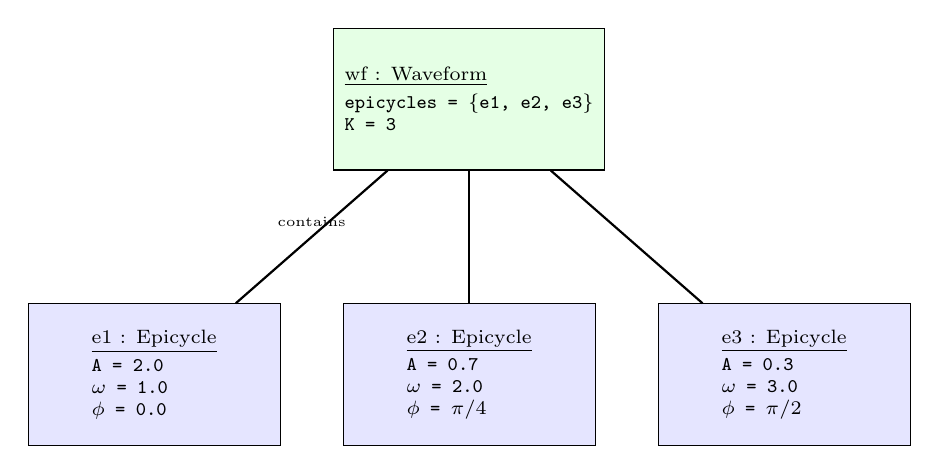
\begin{tikzpicture}[>=stealth,
        obj/.style={draw, rectangle, fill=blue!10, minimum width=3.2cm, minimum height=1.8cm, align=left, font=\scriptsize, inner sep=4pt},
        link/.style={thick}]
        
        \node[obj, fill=green!10] (wf) at (0,2) {
            \underline{wf : Waveform}\\[2pt]
            \texttt{epicycles = \{e1, e2, e3\}}\\
            \texttt{K = 3}
        };
        
        \node[obj] (e1) at (-4,-1.5) {
            \underline{e1 : Epicycle}\\[2pt]
            \texttt{A = 2.0}\\
            \texttt{$\omega$ = 1.0}\\
            \texttt{$\phi$ = 0.0}
        };
        
        \node[obj] (e2) at (0,-1.5) {
            \underline{e2 : Epicycle}\\[2pt]
            \texttt{A = 0.7}\\
            \texttt{$\omega$ = 2.0}\\
            \texttt{$\phi$ = $\pi/4$}
        };
        
        \node[obj] (e3) at (4,-1.5) {
            \underline{e3 : Epicycle}\\[2pt]
            \texttt{A = 0.3}\\
            \texttt{$\omega$ = 3.0}\\
            \texttt{$\phi$ = $\pi/2$}
        };
        
        \draw[link] (wf) -- node[above, font=\tiny] {contains} (e1);
        \draw[link] (wf) -- (e2);
        \draw[link] (wf) -- (e3);
    \end{tikzpicture}
    \caption{UML 对象图。一个 Waveform 实例 \texttt{wf}，包含三个 Epicycle 实例 \texttt{e1}、\texttt{e2}、\texttt{e3}。每个对象显示其运行时字段值，是类图（\cref{fig:uml_functor_hierarchy}）的一个具体实例。}
    \label{fig:uml_object_diagram}
\end{figure}

\newpage

\section{UML 时序图：从数据到 Waveform}

\begin{figure}[htbp]
    \centering
    \begin{tikzpicture}[>=stealth,
        lifeline/.style={draw, fill=blue!10, minimum width=2.2cm, minimum height=0.7cm, align=center, font=\scriptsize\bfseries},
        act/.style={draw, fill=white, minimum width=2.2cm, minimum height=0.5cm, align=center, font=\tiny},
        msg/.style={->, thick, >=stealth}]
        
        \node[lifeline] (user) at (0,0) {建模者};
        \node[lifeline] (samp) at (3,0) {Sampler};
        \node[lifeline] (spec) at (6,0) {Spectrum};
        \node[lifeline] (wave) at (9,0) {Waveform};
        \node[lifeline] (kdi) at (12,0) {KDI 优化器};
        
        \foreach \x in {0,3,6,9,12} {
            \draw[dashed] (\x,-0.5) -- (\x,-7.5);
        }
        
        \draw[msg] (0,-1) -- node[above, font=\tiny] {sample(data)} (3,-1);
        \draw[msg] (3,-1.7) -- node[above, font=\tiny] {fourierTransform(w)} (6,-1.7);
        \draw[msg, dashed] (6,-2.4) -- node[above, font=\tiny] {toWaveform()} (9,-2.4);
        \draw[msg] (9,-3.1) -- node[above, font=\tiny] {参数初始化} (12,-3.1);
        \draw[msg, dashed] (12,-3.8) -- node[above, font=\tiny] {梯度计算} (9,-3.8);
        \draw[msg] (9,-4.5) -- node[above, font=\tiny] {更新 $\{A_k,\omega_k,\phi_k\}$} (12,-4.5);
        \draw[msg, dashed] (12,-5.2) -- node[above, font=\tiny] {收敛？} (9,-5.2);
        \draw[msg] (9,-5.9) -- node[above, font=\tiny] {返回优化后 Waveform} (0,-5.9);
        \draw[msg] (9,-6.6) -- node[above, font=\tiny] {toEpicycle()} (6,-6.6);
    \end{tikzpicture}
    \caption{UML 时序图。从建模者发起采样请求，Sampler 完成频谱分析，Spectrum 转换为 Waveform，KDI 优化器迭代更新参数直至收敛，最终返回优化后的 Waveform 与 Epicycle 分量。}
    \label{fig:uml_sequence}
\end{figure}

\newpage

\section{建模：从实际问题到周期数学模型}

\begin{definition}[建模的步骤]\label{def:modelling_steps}
建模是将实际问题抽象为周期数学模型的系统化流程：
\begin{enumerate}[label=(\roman*)]
    \item \textbf{识别变换群}：确定系统中存在的基本变换及其对称群。
    \item \textbf{识别不变量}：确定系统在变换群作用下的不变量。
    \item \textbf{建立周期函数}：将系统状态变量表示为周期函数（Functor 的子类）。
    \item \textbf{建立周转圆模型}：将周期函数展开为嵌套周转系统（Waveform）。
    \item \textbf{确定耦合关系}：确定子系统间的周期卷积耦合（Convolution）。
\end{enumerate}
\end{definition}

\begin{remark}[建模步骤的完备性（经验观察／研究纲领）]\label{prop:modelling_completeness}
上述五个步骤覆盖了从实际系统到周期数学模型的必要环节；这是\textbf{经验观察／研究纲领}，不是已证定理：「完备」相对于哪一类模型并未定义，也没有给出可验证的判据（例如「任给实际系统的状态-观测映射，五步复合给出与之同构的 Waveform 表示」），故本处只作为方法论约定使用。
五步各自的依据是：步骤 (i)(ii) 确定系统的对称性与不变量，其中\textbf{对称性是周期结构的必要条件}（周期 $\Rightarrow$ 对称，见 \cref{cor:true_logic}），而不变量的识别是刻画轨道间分层的工具，\textbf{不是周期存在的前提}（存在守恒量全为常值的一致周期系统）；步骤 (iii) 将系统状态表示为周期函数（Functor），这是数学建模的核心，见 \cref{def:periodic_series}；步骤 (iv) 将周期函数展开为周转圆（Waveform），这是周期级数表示的关键；步骤 (v) 确定子系统间的周期卷积耦合，见 \cref{def:convolution}。
\end{remark}

\section{数据：采集与预处理}

\begin{definition}[数据采集的周期数学框架]\label{def:data_acquisition}
数据采集使用\textbf{尺度相关采样}模型：采样率 $R(r,\sigma)$ 和采样点数 $N(r,\sigma)$ 由观察者尺度 $\sigma$ 和观察距离 $r$ 决定，其定义与单调性见「离散采样逼近、同余角与置闰」章 \cref{def:dynamic_sampling}、\cref{prop:sampling_monotonicity}。采样定理（\cref{thm:nyquist_shannon_parallel}）保证：当采样率满足奈奎斯特条件时，周期函数可由采样值唯一重建。
\end{definition}

\begin{remark}[动态采样的单调性（引用）]\label{prop:dynamic_sampling_monotonicity}
本命题与「离散采样逼近、同余角与置闰」章 \cref{prop:sampling_monotonicity} 完全相同：对固定 $\sigma>0$，$R$ 与 $N$ 关于距离 $r$ 严格递减；对固定 $r\ge0$，$R$ 与 $N$ 关于尺度 $\sigma$ 严格递增。陈述与证明均见该处，此处不再重复。
\end{remark}

\section{分析：周期卷积与频谱分解}

\begin{definition}[分析的完整工具链]\label{def:analysis_toolchain}
\begin{enumerate}[label=(\roman*)]
    \item \textbf{传统积分变换}：傅里叶、小波、梅林、拉普拉斯、Chirp-Z 变换。
    \item \textbf{相似度变换}（$\alpha=0$）：仅由相位相似度决定（\cref{def:similarity_essence}）。
    \item \textbf{趋势变换}（$\alpha=1$）：由振幅和相位相似度共同决定（\cref{def:tendency}）。
    \item \textbf{权重核}：高斯、墨西哥帽、柯西等核函数（\cref{def:window_function}）。
\end{enumerate}
\end{definition}

\begin{proposition}[分析工具链的包含结构]\label{prop:analysis_hierarchy}
四种分析工具在\textbf{信息保留范围}上构成包含关系（每一后者保留前者的全部信息，并增加新的维度）：
\[
\text{传统变换} \subset \text{趋势变换} \subset \text{相似度变换} \subset \text{权重核}
\]
\end{proposition}

\begin{proof}
（层次 1 $\to$ 层次 2）传统积分变换只给出单函数的频谱系数 $c_k$；趋势变换保留两个函数的振幅和相位交互 $\mathbb{T}_{mn} = A_n B_m e^{i(\phi_n - \psi_m)}$，其对角项退化后即为传统变换（\cref{prop:periodic_transform_vs_classical}）。

（层次 2 $\to$ 层次 3）趋势变换包含振幅乘积 $A_n B_m$；相似度变换丢弃振幅信息，只保留相位关系 $\mathbb{P}_{mn} = e^{i(\phi_n - \psi_m)}$——它是趋势变换在振幅取 $A_n = B_m = 1$ 时的特例。

（层次 3 $\to$ 层次 4）相似度变换对每个频率对 $(n,m)$ 给出相同的相位核；权重核通过窗函数 $W$ 对频率对进行加权，从而在各频率对上实现\textbf{非均匀}的核强度——这是相似度变换所不具备的自由度。

因此四者的信息保留范围构成严格的包含关系。
\end{proof}

\section{处理：窗函数与导-积下降优化}

\begin{definition}[处理的工具]\label{def:processing_tools}
\begin{enumerate}[label=(\roman*)]
    \item \textbf{窗函数平滑}：多尺度平滑，使用高斯核、柯西核等（\cref{def:window_function}）。
    \item \textbf{拐点检测}：使用瞬时极限角的方向变化判据（\cref{def:ts_turning_point,def:limit_angle}）。
    \item \textbf{转折率计算}：拐点两侧正弦趋势之差（\cref{def:ts_refraction}）。
    \item \textbf{导-积下降优化}：核函数导-积下降法（\cref{def:kdi_definition}）。
\end{enumerate}
\end{definition}

\begin{proposition}[处理工具的分工]\label{prop:processing_division}
窗函数平滑负责噪声抑制，拐点检测负责方向转折识别，转折率计算负责转折强度量化，导-积下降优化负责参数精细调整。四种工具协同完成从原始数据到精炼信号的完整处理链。
\end{proposition}

\begin{proof}
每种工具针对信号处理的一个特定方面：
\begin{itemize}
    \item 窗函数平滑（\cref{def:window_function}）：通过卷积 $P * K_\Delta$ 抑制 $|\omega| > 1/\Delta$ 的高频噪声（\cref{ch29_window_spectral}）；
    \item 拐点检测（\cref{def:ts_turning_point}）：通过 $|\theta_t - \theta_{t-1}| > \tau$ 识别方向突变；
    \item 转折率计算（\cref{def:ts_refraction}）：通过 $R_{\text{turn}} = |\sin\theta_1 - \sin\theta_2|$ 量化转折强度；
    \item 导-积下降（\cref{def:kdi_definition}）：通过多核函数融合利用一阶导与积分信息。
\end{itemize}
四者按“平滑 $\to$ 检测 $\to$ 量化 $\to$ 优化”的顺序使用形成完整的处理链。
\end{proof}

\section{评判：模型选择与验证}

\begin{definition}[评判的标准]\label{def:evaluation_criteria}
\begin{enumerate}[label=(\roman*)]
    \item \textbf{信息准则}：AIC、BIC。
    \item \textbf{交叉验证}：$k$ 折交叉验证。
    \item \textbf{残差诊断}：多核函数诊断（\cref{prop:ts_residual_diagnosis}）。
    \item \textbf{贝叶斯模型选择}：后验概率比较（\cref{def:bayesian_inference}）。
\end{enumerate}
\end{definition}

\begin{proposition}[BIC 的拟合-复杂度平衡]\label{prop:bic_balance}
BIC 准则 $\operatorname{BIC}(K) = n\ln(\operatorname{RSS}/n) + K\ln n$ 中，第一项度量拟合优度，第二项惩罚模型复杂度。当 $n$ 增大时，复杂度惩罚的相对权重增加。
\end{proposition}

\begin{proof}
第一项 $n\ln(\operatorname{RSS}/n)$ 随残差减小而减小。第二项 $K\ln n$ 随周转圆级数 $K$ 线性增加。当样本量 $n$ 增大时，$\ln n$ 增大，复杂度惩罚的绝对值和相对权重均增加，使得 BIC 在大样本下更倾向于选择简约模型。严格的最优 $K$ 选择由 \cref{ch34_pipeline_closure} 保证。
\end{proof}

\section{周期：识别与验证}

\begin{definition}[周期识别的判据]\label{def:period_identification}
\begin{enumerate}[label=(\roman*)]
    \item \textbf{频谱峰值}：傅里叶系数的显著峰（\cref{prop:ts_period_significance}）。
    \item \textbf{自相关峰值}：互相关在时延 $T$ 处的峰。
    \item \textbf{相位一致性}：相位算子的闭合性（\cref{def:discrete_phase_operator}）。
    \item \textbf{显著性检验}：Fisher 检验（\cref{prop:ts_period_significance}）。
\end{enumerate}
\end{definition}

\begin{proposition}[Fisher 检验的阈值]\label{prop:fisher_threshold}
Fisher 检验统计量及其显著性阈值的首次陈述见第~\ref{chap:ts_analysis}~章 \cref{sec:ts_period_determination} 中的 \cref{prop:ts_period_significance}；本处为同一结论在建模流程中的复用。
设周期图在 $m = \lfloor (n-1)/2 \rfloor$ 个正频率点上的取值为 $I_1, \dots, I_m$。Fisher 检验统计量
\[
g = \frac{\max_k I_k}{\sum_{k=1}^{m} I_k}
\]
的显著性阈值为 $g_\alpha = 1 - (\alpha/m)^{1/(m-1)}$。
\end{proposition}

\begin{proof}
白噪声下周期图纵坐标独立同分布于指数分布，归一化比值服从 $\operatorname{Beta}(1, m-1)$ 分布。并集界给出 $\mathbb{P}(g > g_0) \le m(1-g_0)^{m-1}$。令右端等于 $\alpha$ 解得 $g_\alpha$。
\end{proof}

\section{周转圆：嵌套结构与参数估计}

\begin{definition}[周转圆建模]\label{def:epicycle_modelling}
$K$ 级嵌套周转系统（Waveform）：
\[
X(t) = \sum_{k=1}^{K} A_k e^{i(\omega_k t + \phi_k)} + \varepsilon(t).
\]
参数估计流程：FFT 初始估计，然后导-积下降精细优化，最后 BIC 模型选择。
\end{definition}

\begin{property}[周转圆模型的基本性质]\label{ch34_epicycle_properties}
\begin{enumerate}[label=(\roman*)]
    \item \textbf{线性叠加}：两级周转圆模型之和仍是周转圆模型。
    \item \textbf{参数可辨识性}：频率两两互异时，振幅与相位由玻尔均值唯一确定。
    \item \textbf{嵌套不变性}：模型在时间平移下形式不变。
\end{enumerate}
\end{property}

\begin{proof}
(i) 两个有限和的逐项合并仍是有限和（\cref{prop:epicycle-closure}(i)）。

(ii) 由玻尔唯一性定理（\cref{thm:periodic_series_bohr}），频率互异时玻尔均值唯一提取各分量系数。

(iii) 时间平移 $t \mapsto t + t_0$ 仅使相位变为 $\phi_k + \omega_k t_0$，形式不变（\cref{prop:epicycle-closure}(ii)）。
\end{proof}

\section{Waveform：周转圆作为复变函数}

\begin{definition}[Waveform：周转圆作为复变函数]\label{def:waveform_definition}
一个 \textbf{Waveform} 是一个复变函数（Functor 的子类），它将时间映射到复平面上的点：
\[
\mathcal{W}: \mathbb{R} \to \mathbb{C}, \quad \mathcal{W}(t) = \sum_{k=1}^{K} A_k e^{i(\omega_k t + \phi_k)}.
\]
其中 $A_k \in \mathbb{R}^+$ 是振幅，$\omega_k \in \mathbb{R}$ 是角频率，$\phi_k \in [0, 2\pi)$ 是初始相位。
\end{definition}

\begin{property}[Waveform 的基本性质]\label{prop:waveform_properties}
\begin{enumerate}[label=(\roman*)]
    \item \textbf{闭合性}：两个 Waveform 的和仍是一个 Waveform。
    \item \textbf{卷积闭合性}：两个 Waveform 的周期卷积仍是一个 Waveform。
    \item \textbf{时间平移}：$\mathcal{W}(t + t_0)$ 对应相位平移。
    \item \textbf{缩放}：$\mathcal{W}(\lambda t)$ 对应频率缩放。
    \item \textbf{旋转}：$e^{i\theta} \mathcal{W}(t)$ 对应全局相位旋转。
\end{enumerate}
\end{property}

\begin{proof}
(i) 由 \cref{prop:epicycle-closure}(i) 直接推广。

(ii) 两个 Waveform 的周期卷积（\cref{def:periodic_convolution}）给出频率合成 $\omega_k + \nu_l$ 与相位合成 $\phi_k + \psi_l$，仍是同形式复指数之和。

(iii) 由 \cref{prop:epicycle-closure}(ii)。

(iv) 由 \cref{prop:epicycle-closure}(iii)。

(v) 由 \cref{prop:epicycle-closure}(iv)。
\end{proof}

\begin{definition}[复指数激活函数：Waveform 的激活函数实现]\label{def:eaf_methodology}
Waveform 的激活函数实现将嵌套周转系统实现为可学习的复变函数：
\[
\mathcal{E}(x) = \sum_{k=1}^{N} A_k e^{i(\omega_k x + \phi_k)}.
\]
参数 $A_k$、$\omega_k$、$\phi_k$ 可通过反向传播或导-积下降优化学习。其数学对象即第~\ref{chap:epicycle-activation}~章 \cref{def:epicycle-activation} 定义的周转圆激活函数。
\end{definition}

\begin{proposition}[导-积下降：Waveform 参数的优化器]\label{prop:kdi_methodology}
Waveform 参数优化的导-积下降策略：
\begin{center}
\begin{tabular}{@{}p{2.5cm} p{2.5cm} p{2.5cm} p{4cm}@{}}
\toprule
参数 & 核函数 & 算子偏向 & 优化特性 \\
\midrule
振幅 $A_k$ & 高斯核 & 梯度（对称中心 $0$） & 光滑调整 \\
频率 $\omega_k$ & 墨西哥帽核 & 旋度（对称中心 $i$） & 曲率感知 \\
相位 $\phi_k$ & Hilbert 核 & 旋度（对称中心 $i$） & 跳变检测 \\
\bottomrule
\end{tabular}
\end{center}
\end{proposition}

\begin{proof}
高斯核平滑抑制高频噪声，适合振幅的光滑调整（\cref{lem:gaussian_fourier_duality}）。墨西哥帽核为高斯核的二阶导，带通特性凸显频率曲率（\cref{def:window_function}）。Hilbert 核提供 $90^\circ$ 相位旋转，适合相位跳变检测（\cref{def:hilbert}）。
\end{proof}

\begin{figure}[htbp]
    \centering
    \begin{tikzpicture}[>=stealth,
        box/.style={draw, rounded corners, minimum width=2.4cm, minimum height=0.9cm, align=center, font=\small},
        arrow/.style={->, thick, >=stealth}]
        
        \node[box, fill=blue!15] (data) at (0,0) {观测数据\\$X(t)$};
        \node[box, fill=green!15] (fft) at (5,1.5) {频谱\\初步估计};
        \node[box, fill=red!15] (kdi) at (5,-1) {导-积下降\\精细调整};
        \node[box, fill=orange!15] (waveform) at (5,-3) {Waveform 建模\\复变函数};
        \node[box, fill=purple!15] (pred) at (10,0) {预测诊断};
        
        \draw[arrow] (data) -- (fft);
        \draw[arrow] (fft) -- (kdi);
        \draw[arrow] (kdi) -- (waveform);
        \draw[arrow] (waveform) -- (pred);
        \draw[arrow, dashed, blue, thick] (pred.south) -- node[below, font=\footnotesize, yshift=0.8cm] {反馈} (data.south);
    \end{tikzpicture}
    \caption{Waveform 与导-积下降协同流程。}
    \label{fig:waveform_kdi_pipeline}
\end{figure}

\begin{remark}[与全书的统一]\label{rem:methodology_unity}
本章建立的建模与分析框架是周期数学全部理论的方法论整合。核心类体系以 Functor 为统一抽象，分为三个模块：函数类层次结构（Functor + 基本函数 + Epicycle + Waveform + Convolution）、级数类层次结构（Series + Taylor + Fourier + Laurent + Periodic）、积分变换与采样类（Sampler + Sample + Spectrum + Spectral）。

Waveform 作为周转圆复变函数是这一方法论框架的汇聚点。Waveform 及其复指数激活函数实现和导-积下降优化的联合使用，使得周期数学的完整理论体系可以直接应用于神经网络、时间序列分析、信号处理等现代数据科学任务。周期卷积为 Waveform 之间的交互提供了统一的算子框架。

\textbf{与下一章的接口}：本章的 Waveform 定义（\cref{def:waveform_definition}）与 Epicycle 类（\cref{def:epicycle_class}）为「周转圆激活函数与函数逼近」章提供数学对象基础；CEAF 定义（\cref{def:eaf_methodology}）与该章的 \cref{def:epicycle-activation} 是同一数学对象在两种语境下的表达。
\end{remark}

\section*{本章七主题对照表}

\begin{center}
\renewcommand{\arraystretch}{1.3}
\begin{tabular}{@{}p{2.2cm} p{10.5cm}@{}}
\toprule
主题 & 本章对应 \\
\midrule
平移 & 数据采集的时间序列推进与动态采样（\cref{def:data_acquisition}）；Waveform 的时间平移不变性（\cref{prop:waveform_properties}(iii)） \\
缩放 & BIC 的复杂度惩罚 $K\ln n$（\cref{ch34_pipeline_closure}）；多尺度窗函数（\cref{def:processing_tools}）；Waveform 的频率缩放（\cref{prop:waveform_properties}(iv)） \\
旋转 & 周转圆模型的相位 $\phi_k$（\cref{def:epicycle_modelling}）；Waveform 的复变相位表示（\cref{def:waveform_definition}）；全局相位旋转（\cref{prop:waveform_properties}(v)） \\
平衡 & BIC 的拟合-复杂度平衡（\cref{prop:bic_balance}）；玻尔均值的参数唯一性（\cref{ch34_epicycle_properties}(ii)） \\
对称 & 周转圆嵌套的层级对称；模型的时间平移不变性（\cref{ch34_epicycle_properties}(iii)） \\
闭合 & 方法论流程的反馈迭代闭合（\cref{ch34_pipeline_closure}）；Functor 类的闭包性质（\cref{prop:functor_closure}） \\
周期 & 频谱峰值识别（\cref{def:period_identification}）；周转圆参数估计（\cref{def:epicycle_modelling}）；Waveform 的卷积闭合性（\cref{prop:waveform_properties}(ii)） \\
\bottomrule
\end{tabular}
\end{center}

\section*{本章思考题}

\begin{enumerate}[leftmargin=3em, label=\textbf{题 \arabic*}]
    \item 证明本章的\textbf{方法论流程的反馈闭合}（\ref{ch34_pipeline_closure}）。提示：先写出本章目标的判定映射与演化群，再套用「周期系统」章通用判据的证明结构。

    \item 验证\textbf{基本函数的导数封闭性}（\ref{prop:basic_function_derivative_closure}）的前提在本章领域对象上成立，并给出一个不满足前提的反例。

    \item 考察\textbf{Series 与 Waveform 的关系}（\ref{prop:series_waveform_relation}）在参数退化时的行为，说明结论如何随之退化。

    \item 讨论\textbf{建模步骤的完备性}这一方法论约定（\textbf{经验观察／研究纲领}，见注 \ref{prop:modelling_completeness}）与「周期系统」章相应通用结论的关系（是一致、特例还是需要附加条件）。

    \item 根据本章七主题对照表，分别指出本章在\textbf{平移}、\textbf{缩放}、\textbf{旋转}三个主题上的具体载体，并各举一个领域数据实例。

    \item 综合题：用「周期系统」章的五步标准接口（表 \ref{tab:ps_five_steps}）重述本章的诊断流程，并逐一注明每一步所依赖的本章结论：\ref{ch34_pipeline_closure}、\ref{prop:basic_function_derivative_closure}、\ref{prop:series_waveform_relation}、\ref{prop:modelling_completeness}（\textbf{经验观察／研究纲领}）。
\end{enumerate}


